\documentclass[aspectratio=169,10pt]{beamer}

\usepackage[T1]{fontenc}
\usepackage[utf8]{inputenc}
\usepackage[spanish,es-tabla]{babel}
\usepackage{lmodern}
\usepackage{graphicx}
\usepackage{booktabs}
\usepackage{array}
\usepackage{tikz}
\usetikzlibrary{arrows.meta,positioning}

\graphicspath{{results/figures/}}

\definecolor{Ink}{HTML}{173042}
\definecolor{Energy}{HTML}{0C6670}
\definecolor{EnergySoft}{HTML}{DCEDEF}
\definecolor{Amber}{HTML}{D98E32}
\definecolor{Paper}{HTML}{FAF8F2}
\definecolor{Muted}{HTML}{5D6B73}
\definecolor{Alert}{HTML}{B85750}

\setbeamercolor{normal text}{fg=Ink,bg=Paper}
\setbeamercolor{frametitle}{fg=Ink,bg=Paper}
\setbeamercolor{title}{fg=Ink}
\setbeamercolor{subtitle}{fg=Energy}
\setbeamercolor{structure}{fg=Energy}
\setbeamercolor{block title}{fg=Paper,bg=Energy}
\setbeamercolor{block body}{fg=Ink,bg=EnergySoft}
\setbeamercolor{alerted text}{fg=Alert}
\setbeamercolor{footline}{fg=Muted,bg=Paper}
\setbeamerfont{frametitle}{series=\bfseries,size=\large}
\setbeamerfont{title}{series=\bfseries,size=\LARGE}
\setbeamersize{text margin left=0.65cm,text margin right=0.65cm}

\setbeamertemplate{navigation symbols}{}
\setbeamertemplate{itemize item}{\color{Amber}\small$\blacktriangleright$}
\setbeamertemplate{itemize subitem}{\color{Energy}\scriptsize$\bullet$}
\setbeamertemplate{frametitle}{
  \vspace{0.28cm}
  \begin{beamercolorbox}[wd=\paperwidth,leftskip=0.65cm,rightskip=0.65cm]{frametitle}
    \usebeamerfont{frametitle}\insertframetitle
  \end{beamercolorbox}
  \vspace{-0.20cm}
  \hspace{0.65cm}{\color{Amber}\rule{0.88\paperwidth}{0.8pt}}
}
\setbeamertemplate{footline}{
  \leavevmode
  \hbox{%
    \begin{beamercolorbox}[wd=\paperwidth,ht=2.8ex,dp=1.2ex,leftskip=0.65cm,rightskip=0.55cm]{footline}
      \scriptsize Proyecto final · Series Temporales\hfill\insertframenumber/10
    \end{beamercolorbox}%
  }
}

\newcommand{\highlight}[1]{\textcolor{Energy}{\textbf{#1}}}
\newcommand{\smallnote}[1]{{\scriptsize\textcolor{Muted}{#1}}}
\newcommand{\metricbox}[2]{
  \begin{beamercolorbox}[rounded=true,sep=0.20cm,center,wd=\linewidth]{block body}
    {\scriptsize\textcolor{Muted}{#1}}\\[-0.02cm]
    {\Large\textbf{#2}}
  \end{beamercolorbox}
}

\title{Forecasting de producción eléctrica mensual}
\author{Juan Daniel Barboza}
\institute{Maestría en Ciencias de la Inteligencia Artificial}
\date{Proyecto final · Series Temporales}

\begin{document}

% 1
\begin{frame}
  \vspace{0.30cm}
  {\usebeamerfont{title}\color{Ink}\inserttitle}\par
  \vspace{0.12cm}
  {\large\color{Energy}\insertsubtitle}\par
  \vspace{0.30cm}
  {\small\insertauthor}\par
  {\scriptsize\color{Muted}\insertinstitute}

  \vfill
  \begin{block}{Pregunta central}
    \large ¿Un modelo con estructura estacional explícita puede superar a Machine Learning y a una referencia anual simple?
  \end{block}

  \vspace{0.20cm}
  \begin{columns}[T,onlytextwidth]
    \column{0.31\textwidth}
      \metricbox{Serie mensual}{397 observaciones}
    \column{0.31\textwidth}
      \metricbox{Horizonte final}{24 meses}
    \column{0.31\textwidth}
      \metricbox{Modelos comparados}{2 categorías}
  \end{columns}
\end{frame}

% 2
\begin{frame}{Problema y dataset}
  \begin{columns}[T,onlytextwidth]
    \column{0.40\textwidth}
      \begin{block}{Objetivo}
        Pronosticar el índice mensual de producción eléctrica \texttt{IPG2211A2N} a partir de su historial.
      \end{block}
      \begin{itemize}
        \item \highlight{397 meses}: 1985--2018.
        \item Frecuencia mensual y objetivo positivo.
        \item Sin faltantes ni fechas duplicadas.
        \item Es un \highlight{índice}, no energía en unidades físicas.
      \end{itemize}
      \smallnote{Fuente: Time Series Datasets (Kaggle). Equivalente: FRED IPG2211A2N.}
    \column{0.57\textwidth}
      \centering
      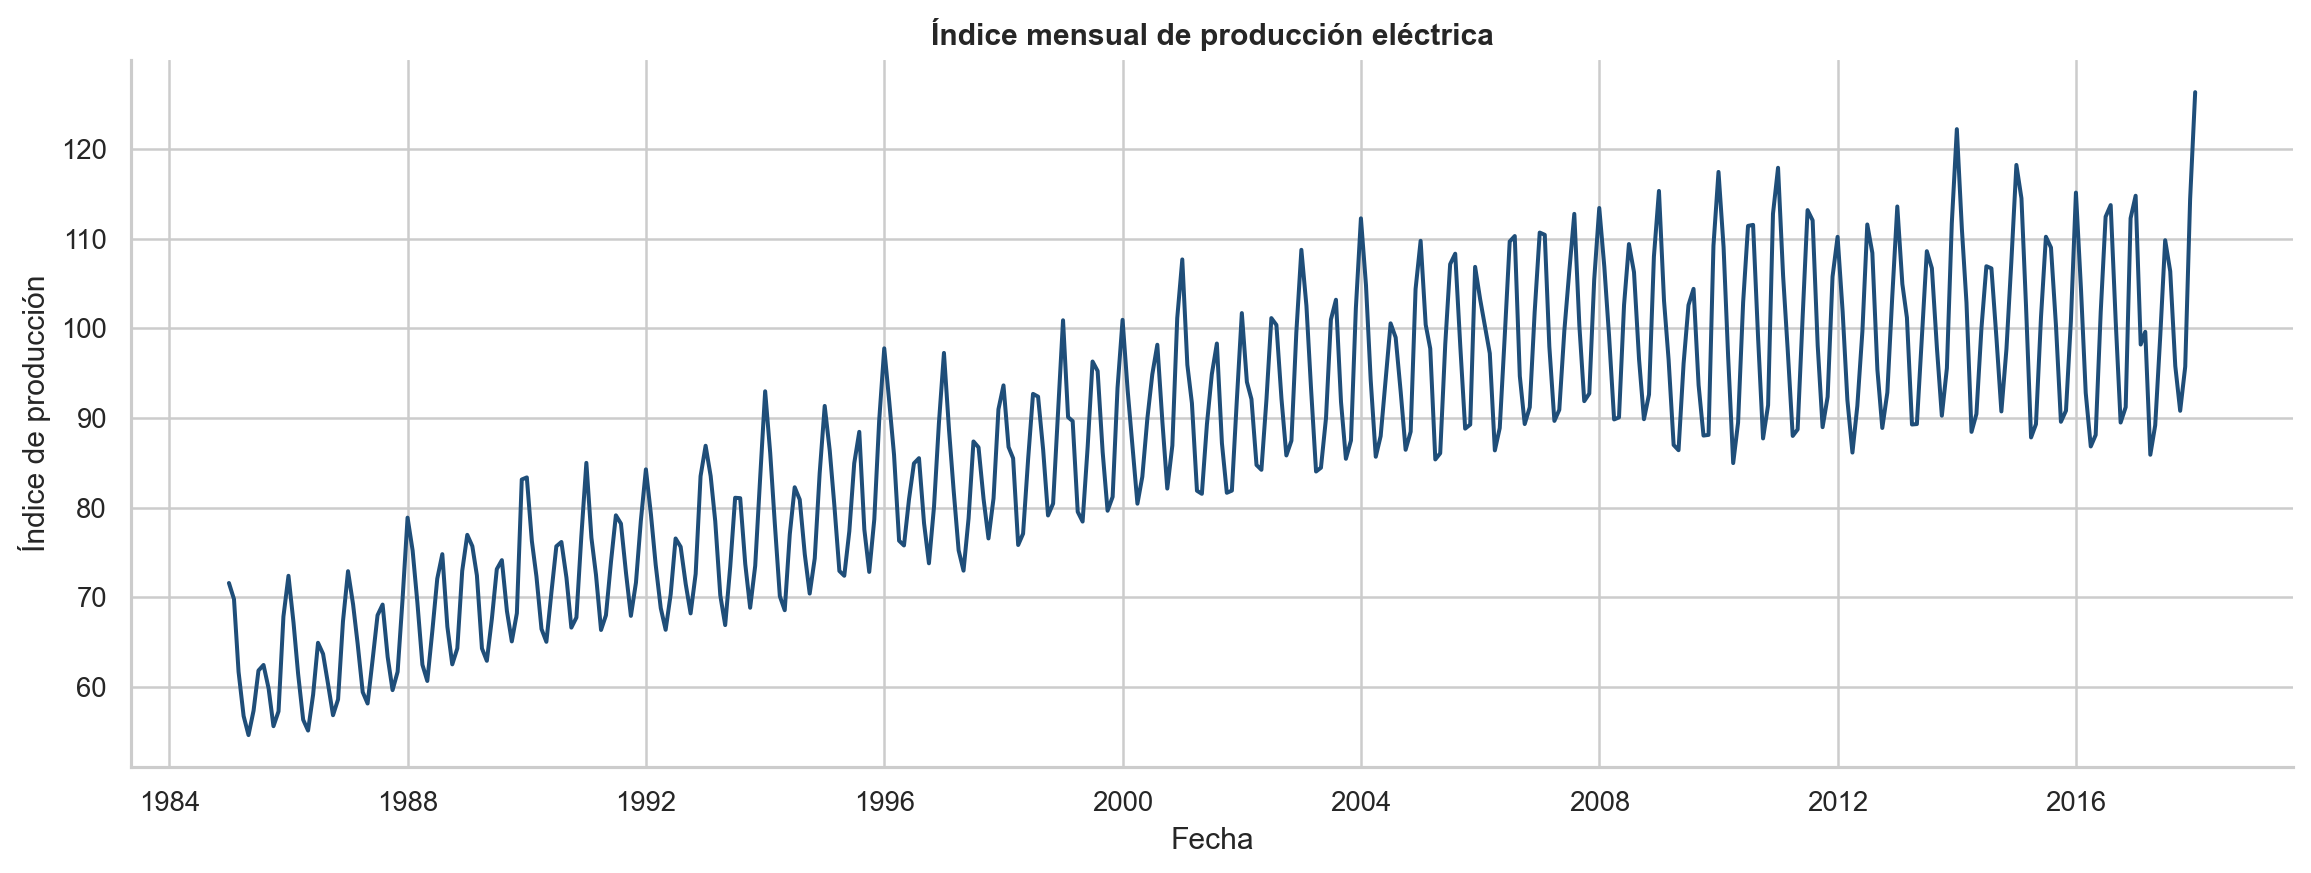
\includegraphics[width=\linewidth,height=0.62\paperheight,keepaspectratio]{01_serie_original.png}
  \end{columns}
\end{frame}

% 3
\begin{frame}{Qué aprendimos de la serie}
  \begin{columns}[T,onlytextwidth]
    \column{0.66\textwidth}
      \centering
      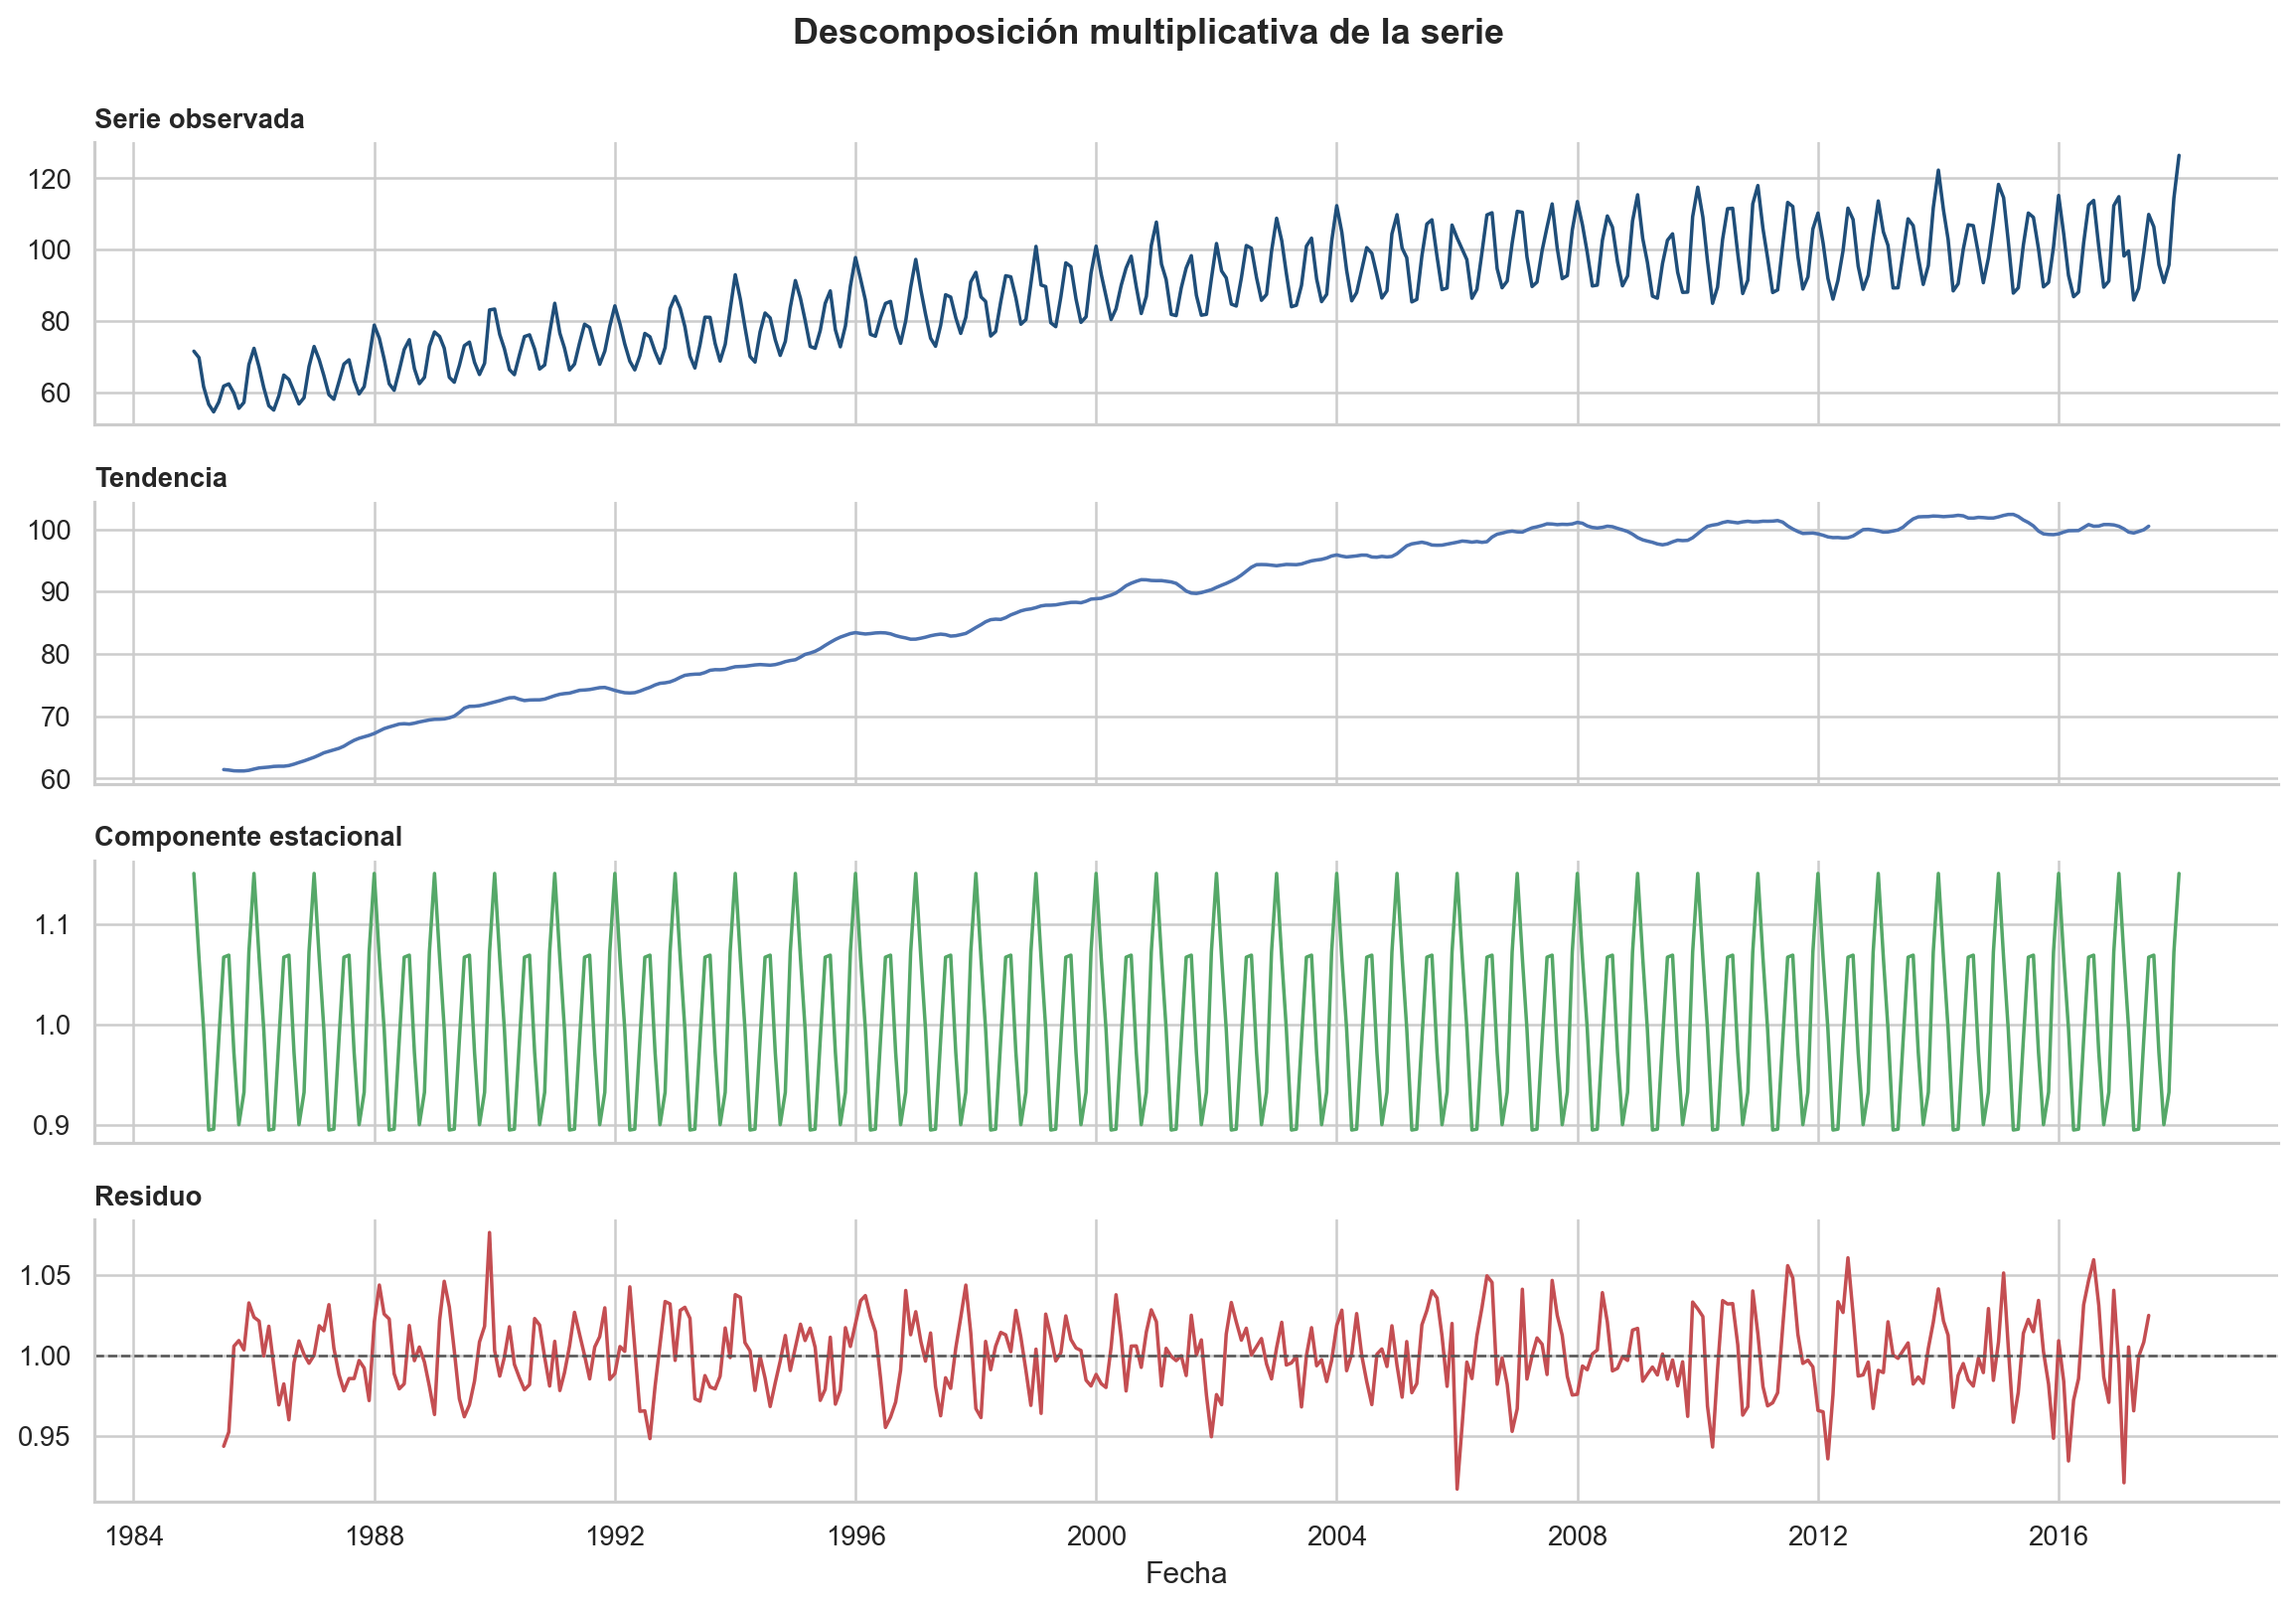
\includegraphics[width=\linewidth,height=0.62\paperheight,keepaspectratio]{03_descomposicion.png}
    \column{0.31\textwidth}
      \begin{block}{Tres señales}
        \begin{itemize}
          \item Tendencia creciente de largo plazo.
          \item Estacionalidad anual clara: período \highlight{12}.
          \item Amplitud asociada al nivel de la serie.
        \end{itemize}
      \end{block}
      \vspace{0.10cm}
      \begin{block}{Decisión}
        Ajustar sobre $\log(y)$ y volver a la escala original antes de medir errores.
      \end{block}
  \end{columns}
\end{frame}

% 4
\begin{frame}{Protocolo temporal}
  \centering
  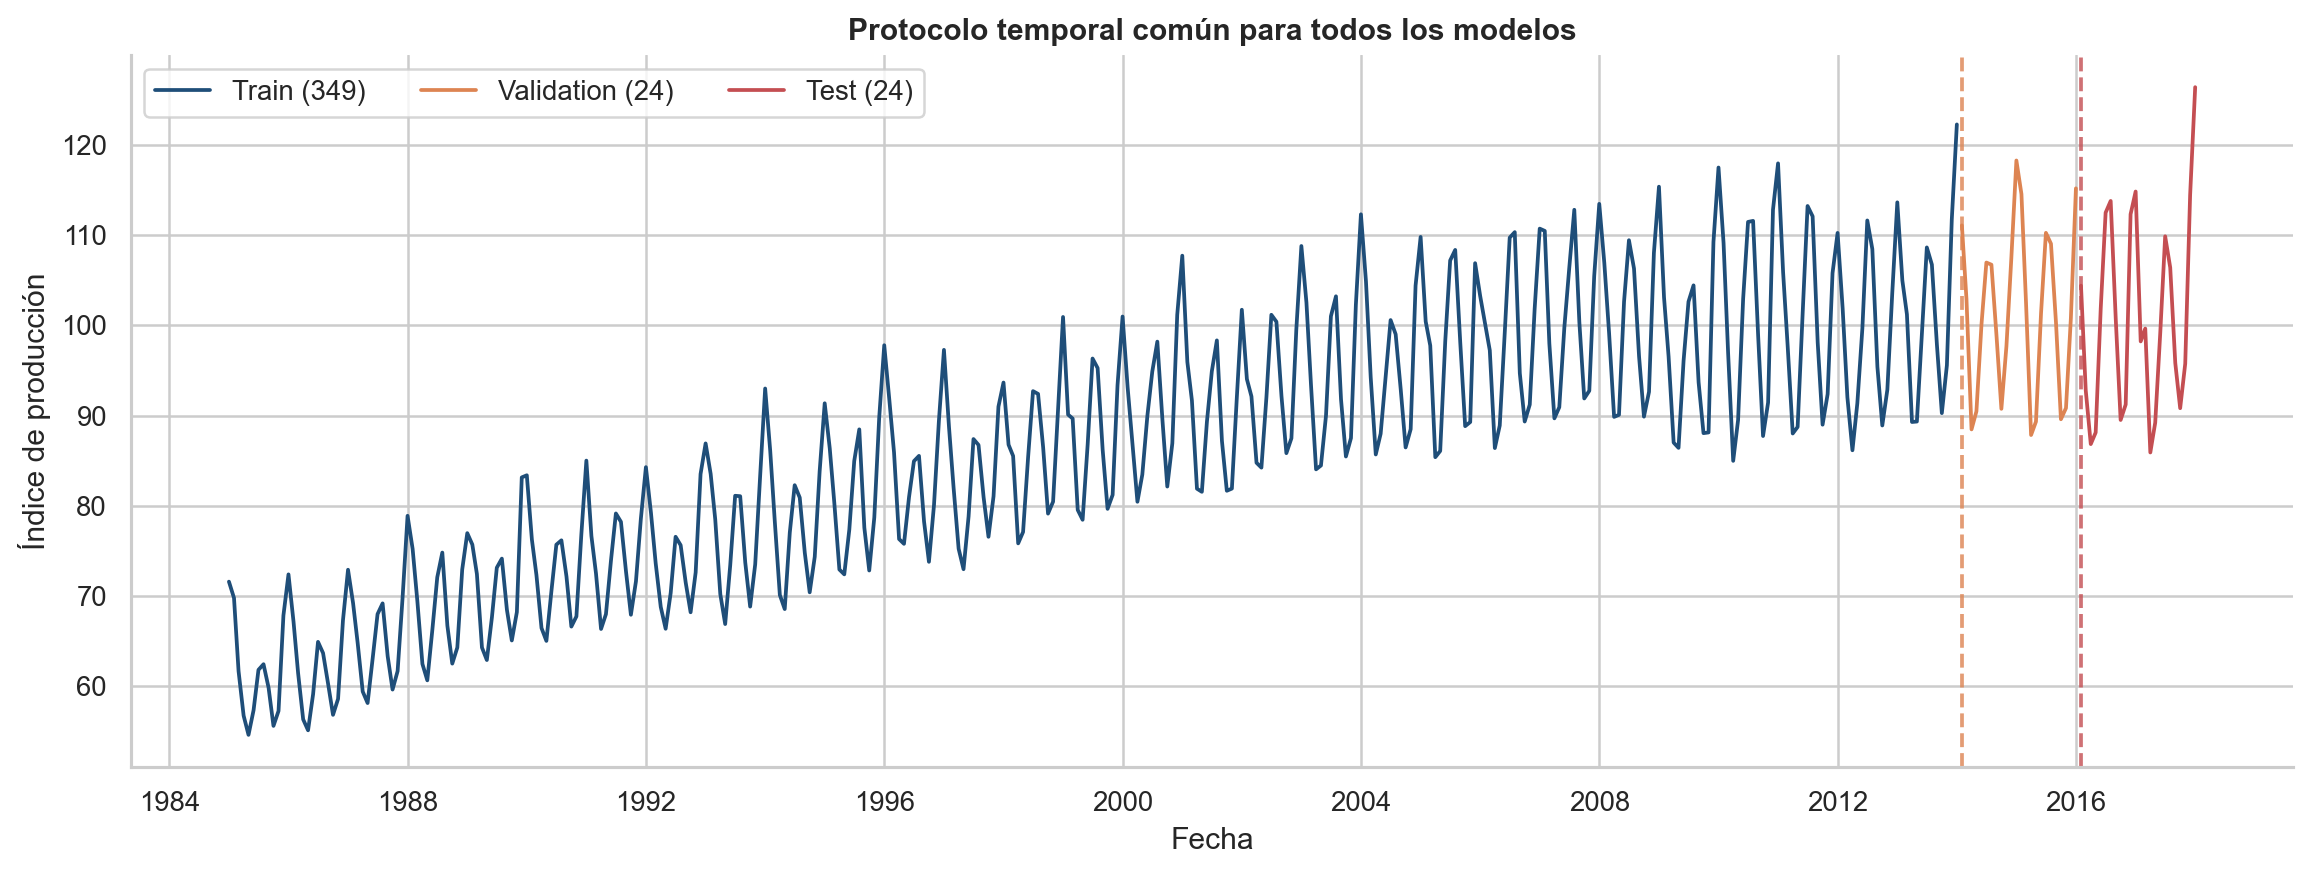
\includegraphics[width=0.92\textwidth,height=0.42\paperheight,keepaspectratio]{05_splits_temporales.png}

  \vspace{0.10cm}
  \begin{columns}[T,onlytextwidth]
    \column{0.47\textwidth}
      \begin{table}
        \centering
        \scriptsize
        \begin{tabular}{lrl}
          \toprule
          Segmento & $n$ & Uso \\
          \midrule
          Train & 349 & Ajustar candidatos \\
          Validation & 24 & Seleccionar \\
          Test & 24 & Evaluar una vez \\
          \bottomrule
        \end{tabular}
      \end{table}
    \column{0.50\textwidth}
      \begin{block}{Control metodológico}
        Mismo historial, mismo origen y mismo horizonte de 24 meses para todos. No se comparan ventanas con distinto número de folds ni fechas iniciales diferentes.
      \end{block}
  \end{columns}
\end{frame}

% 5
\begin{frame}{Modelos y pipeline de pronóstico}
  \centering
  \begin{tikzpicture}[
    node distance=0.48cm,
    box/.style={draw=Energy,fill=EnergySoft,rounded corners=3pt,minimum width=2.35cm,minimum height=0.72cm,align=center,font=\scriptsize},
    arrow/.style={-{Stealth[length=2.3mm]},thick,color=Energy}
  ]
    \node[box] (series) {Serie mensual\\validada};
    \node[box,right=of series] (log) {Transformación\\$\log(y)$};
    \node[box,right=of log] (select) {Selección solo\\en validation};
    \node[box,right=of select] (refit) {Reentrenamiento\\train + validation};
    \node[box,right=of refit] (test) {Pronóstico\\test};
    \draw[arrow] (series)--(log);
    \draw[arrow] (log)--(select);
    \draw[arrow] (select)--(refit);
    \draw[arrow] (refit)--(test);
  \end{tikzpicture}

  \vspace{0.35cm}
  \begin{columns}[T,onlytextwidth]
    \column{0.32\textwidth}
      \begin{block}{Referencia}
        \textbf{Naive estacional}: repite el valor observado 12 meses antes.
      \end{block}
    \column{0.32\textwidth}
      \begin{block}{SARIMA · estadístico}
        Seleccionado: \highlight{$(2,0,2)(1,1,1)_{12}$}. Modela dependencia y estacionalidad explícitamente.
      \end{block}
    \column{0.32\textwidth}
      \begin{block}{XGBoost · ML}
        15 variables: rezagos, ventanas móviles y calendario. Pronóstico \highlight{recursivo} sin valores futuros reales.
      \end{block}
  \end{columns}
\end{frame}

% 6
\begin{frame}{Selección en validation}
  \begin{columns}[T,onlytextwidth]
    \column{0.64\textwidth}
      \centering
      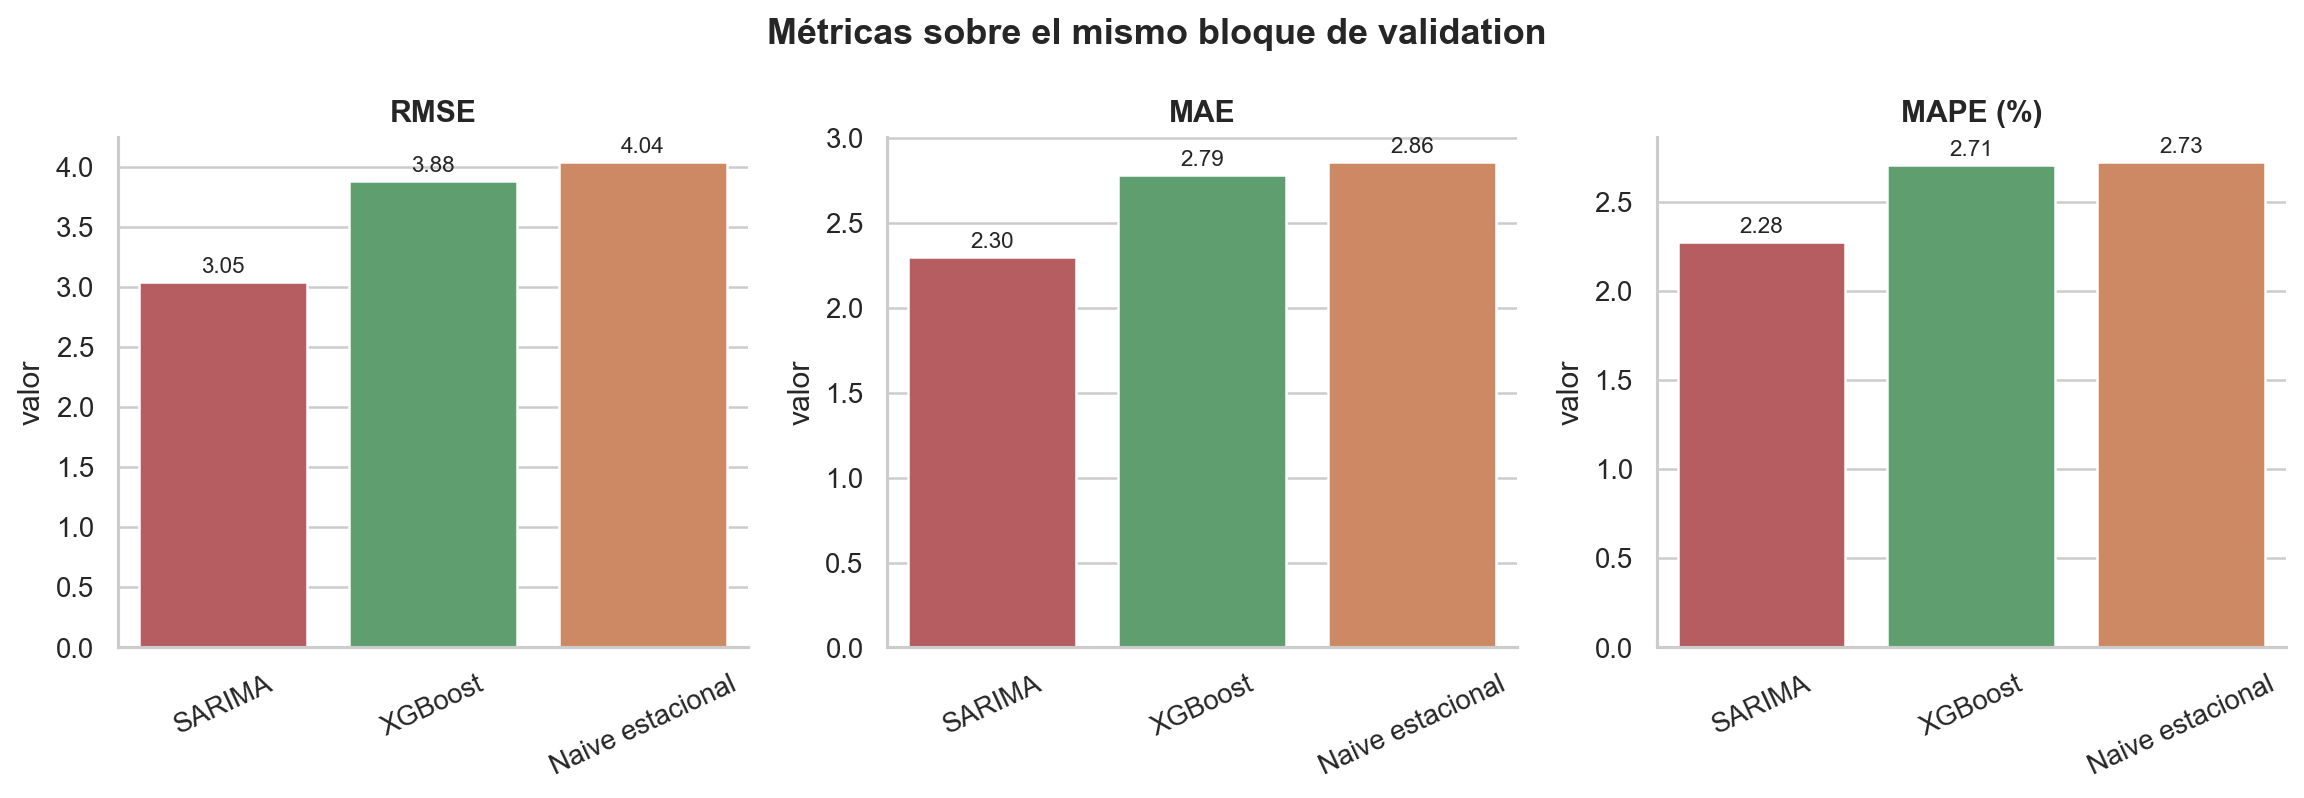
\includegraphics[width=\linewidth,height=0.64\paperheight,keepaspectratio]{11_metricas_validation.png}
    \column{0.33\textwidth}
      \begin{block}{Resultado}
        SARIMA fue mejor en las tres métricas:
        \begin{itemize}
          \item RMSE: \highlight{3,0453}
          \item MAE: \highlight{2,3011}
          \item MAPE: \highlight{2,2756\%}
        \end{itemize}
      \end{block}
      \vspace{0.12cm}
      \smallnote{Se evaluaron 144 configuraciones SARIMA y 64 de XGBoost. La decisión quedó fijada antes de abrir test.}
  \end{columns}
\end{frame}

% 7
\begin{frame}{Pronóstico final sobre test}
  \centering
  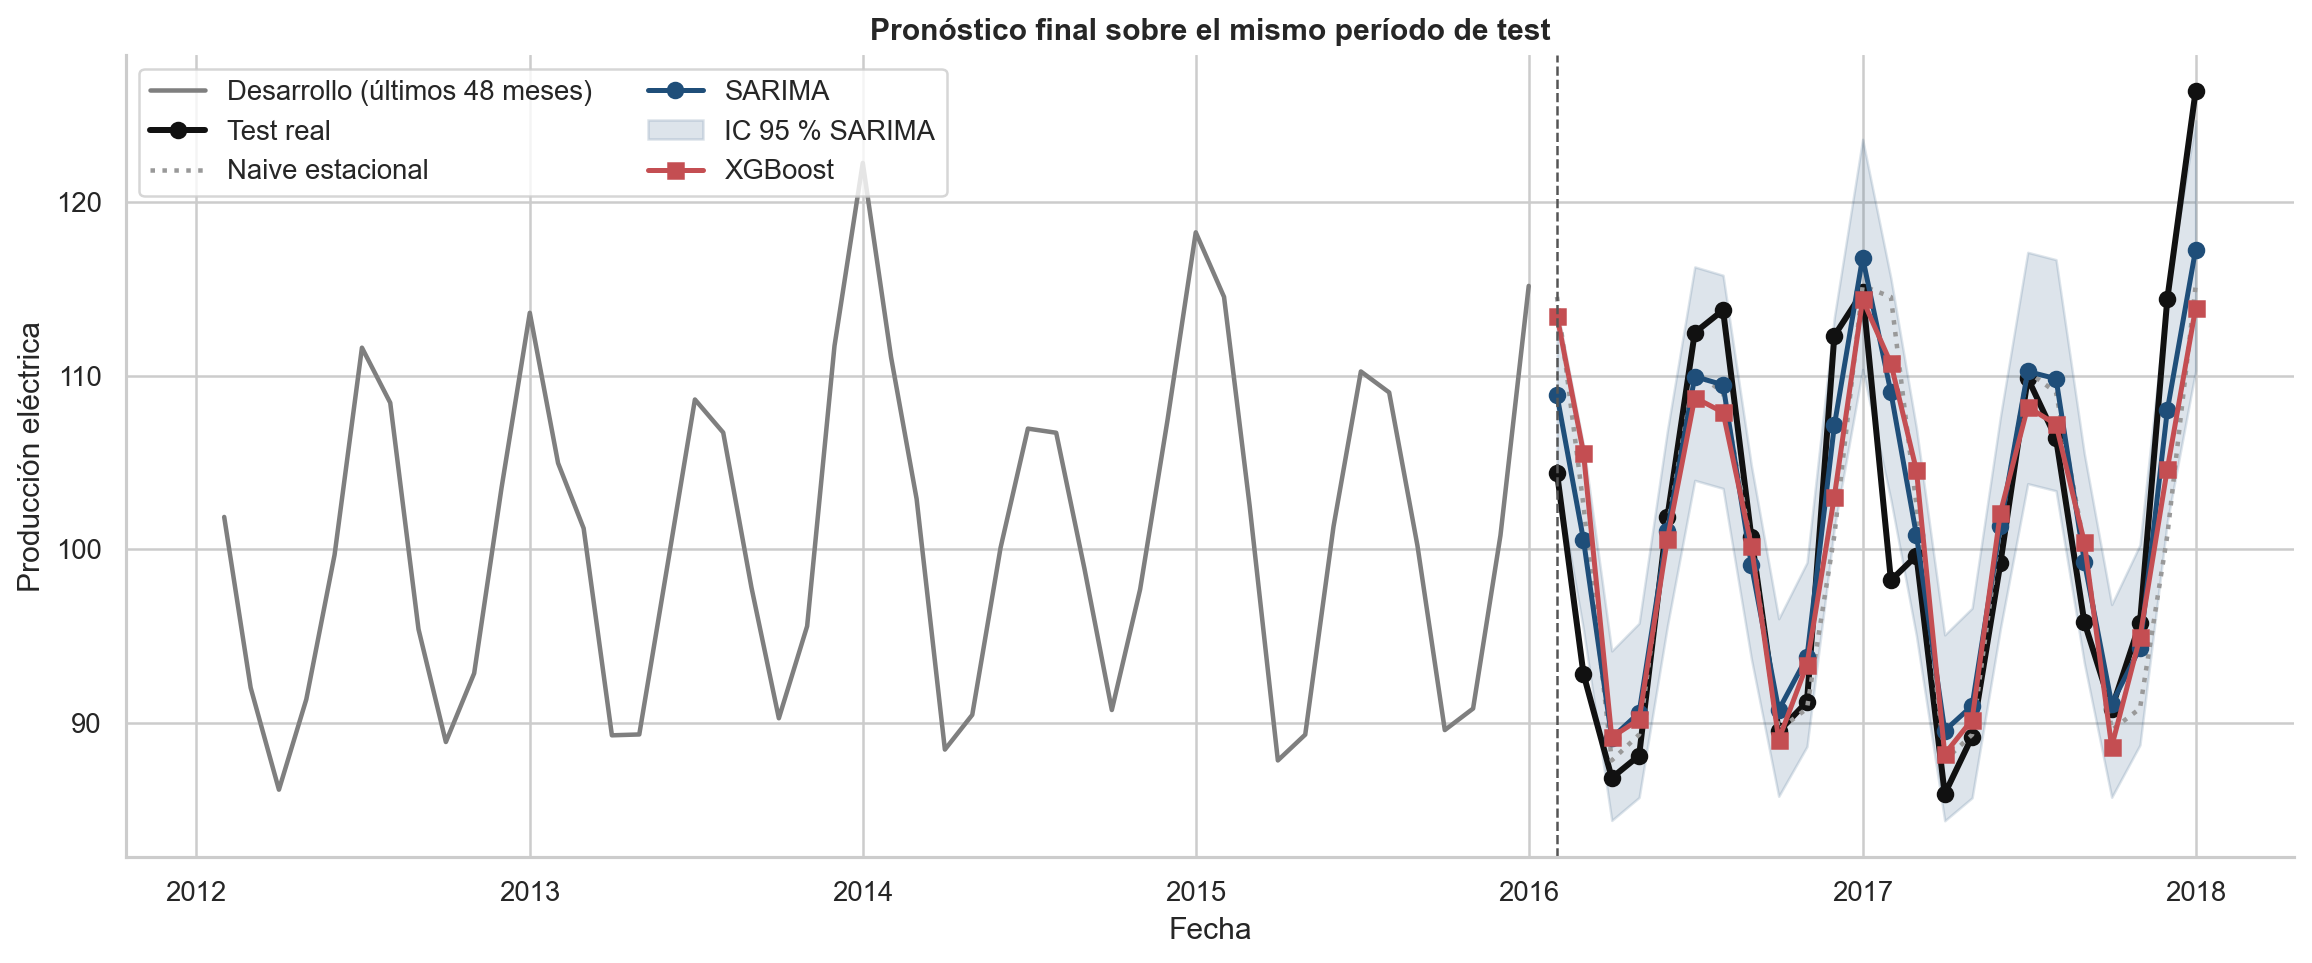
\includegraphics[width=0.96\textwidth,height=0.66\paperheight,keepaspectratio]{13_pronosticos_test.png}

  \vspace{0.05cm}
  \smallnote{Los dos modelos siguen la estacionalidad; XGBoost suaviza más los extremos. La banda corresponde al intervalo de confianza del 95\% de SARIMA.}
\end{frame}

% 8
\begin{frame}{Comparación final de métricas}
  \begin{columns}[T,onlytextwidth]
    \column{0.67\textwidth}
      \centering
      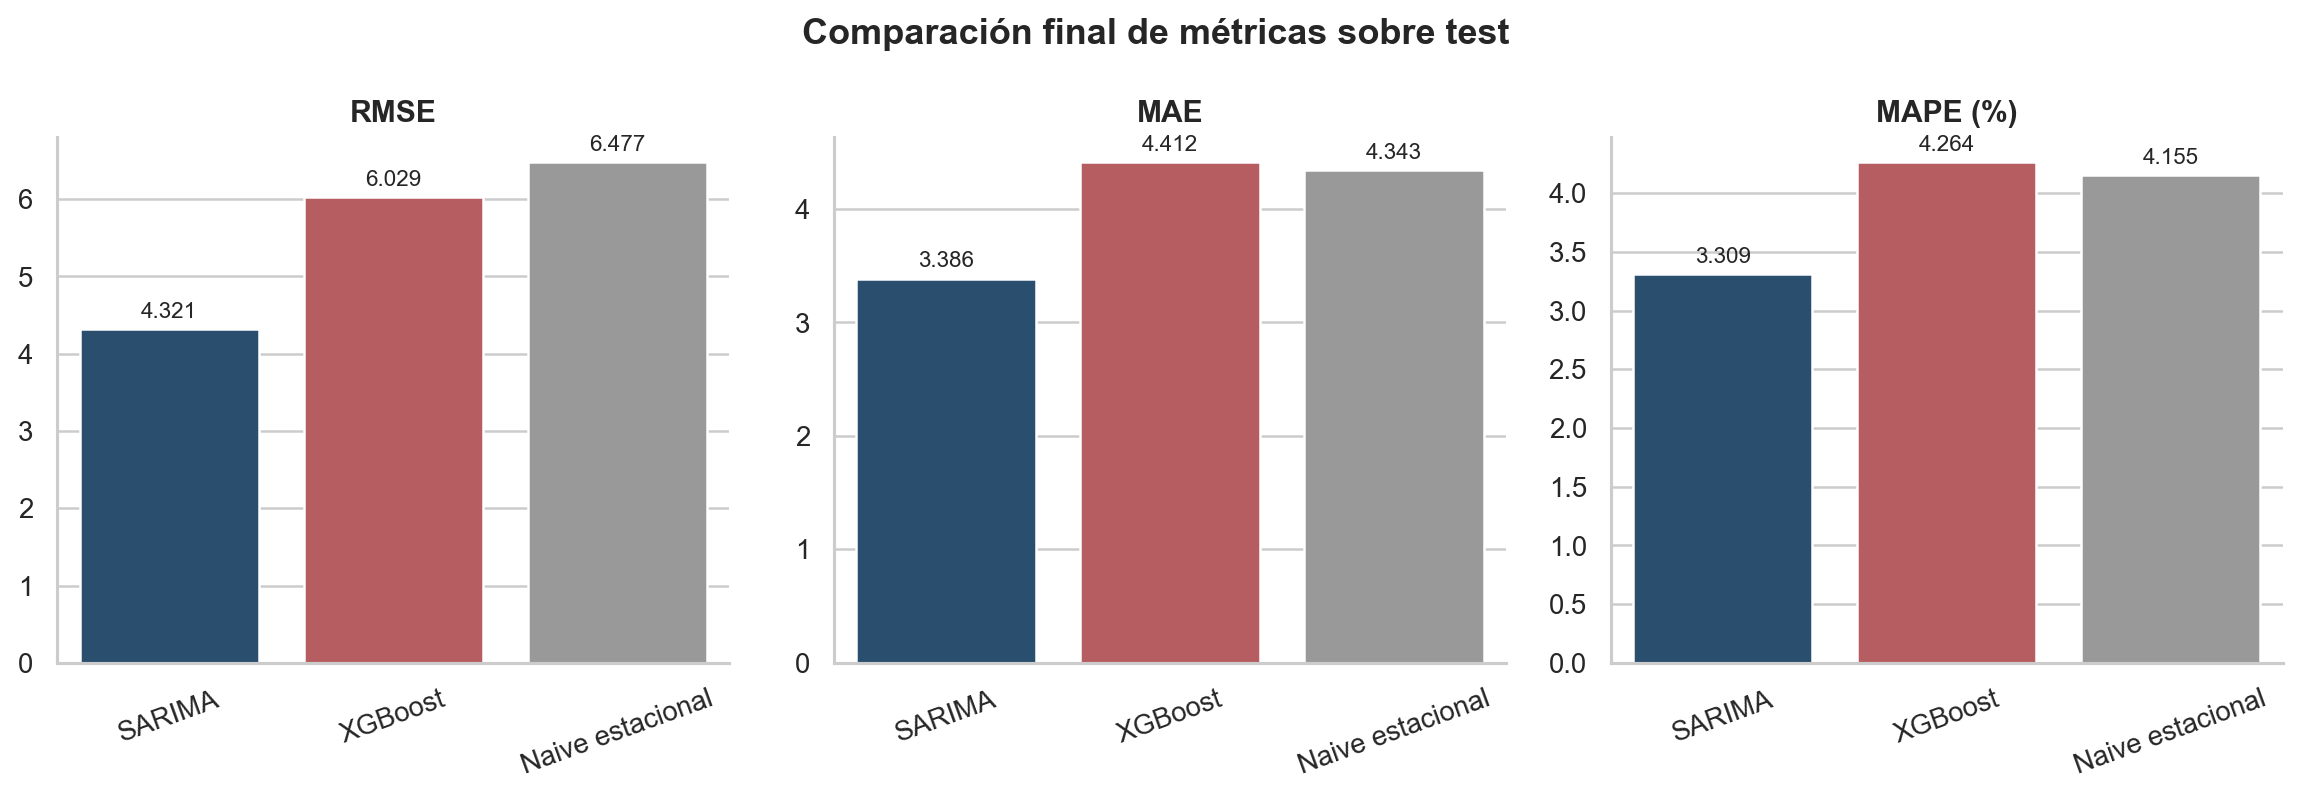
\includegraphics[width=\linewidth,height=0.64\paperheight,keepaspectratio]{14_metricas_test.png}
    \column{0.30\textwidth}
      \begin{block}{SARIMA vs. baseline}
        \begin{itemize}
          \item RMSE: \highlight{$-33,29\%$}
          \item MAE: \highlight{$-22,03\%$}
          \item MAPE: \highlight{$-20,35\%$}
        \end{itemize}
      \end{block}
      \vspace{0.12cm}
      \begin{alertblock}{Lectura de XGBoost}
        Reduce RMSE, pero queda levemente peor que el baseline en MAE y MAPE: la mejora no es consistente.
      \end{alertblock}
  \end{columns}
\end{frame}

% 9
\begin{frame}{Diagnóstico de errores de SARIMA}
  \begin{columns}[T,onlytextwidth]
    \column{0.70\textwidth}
      \centering
      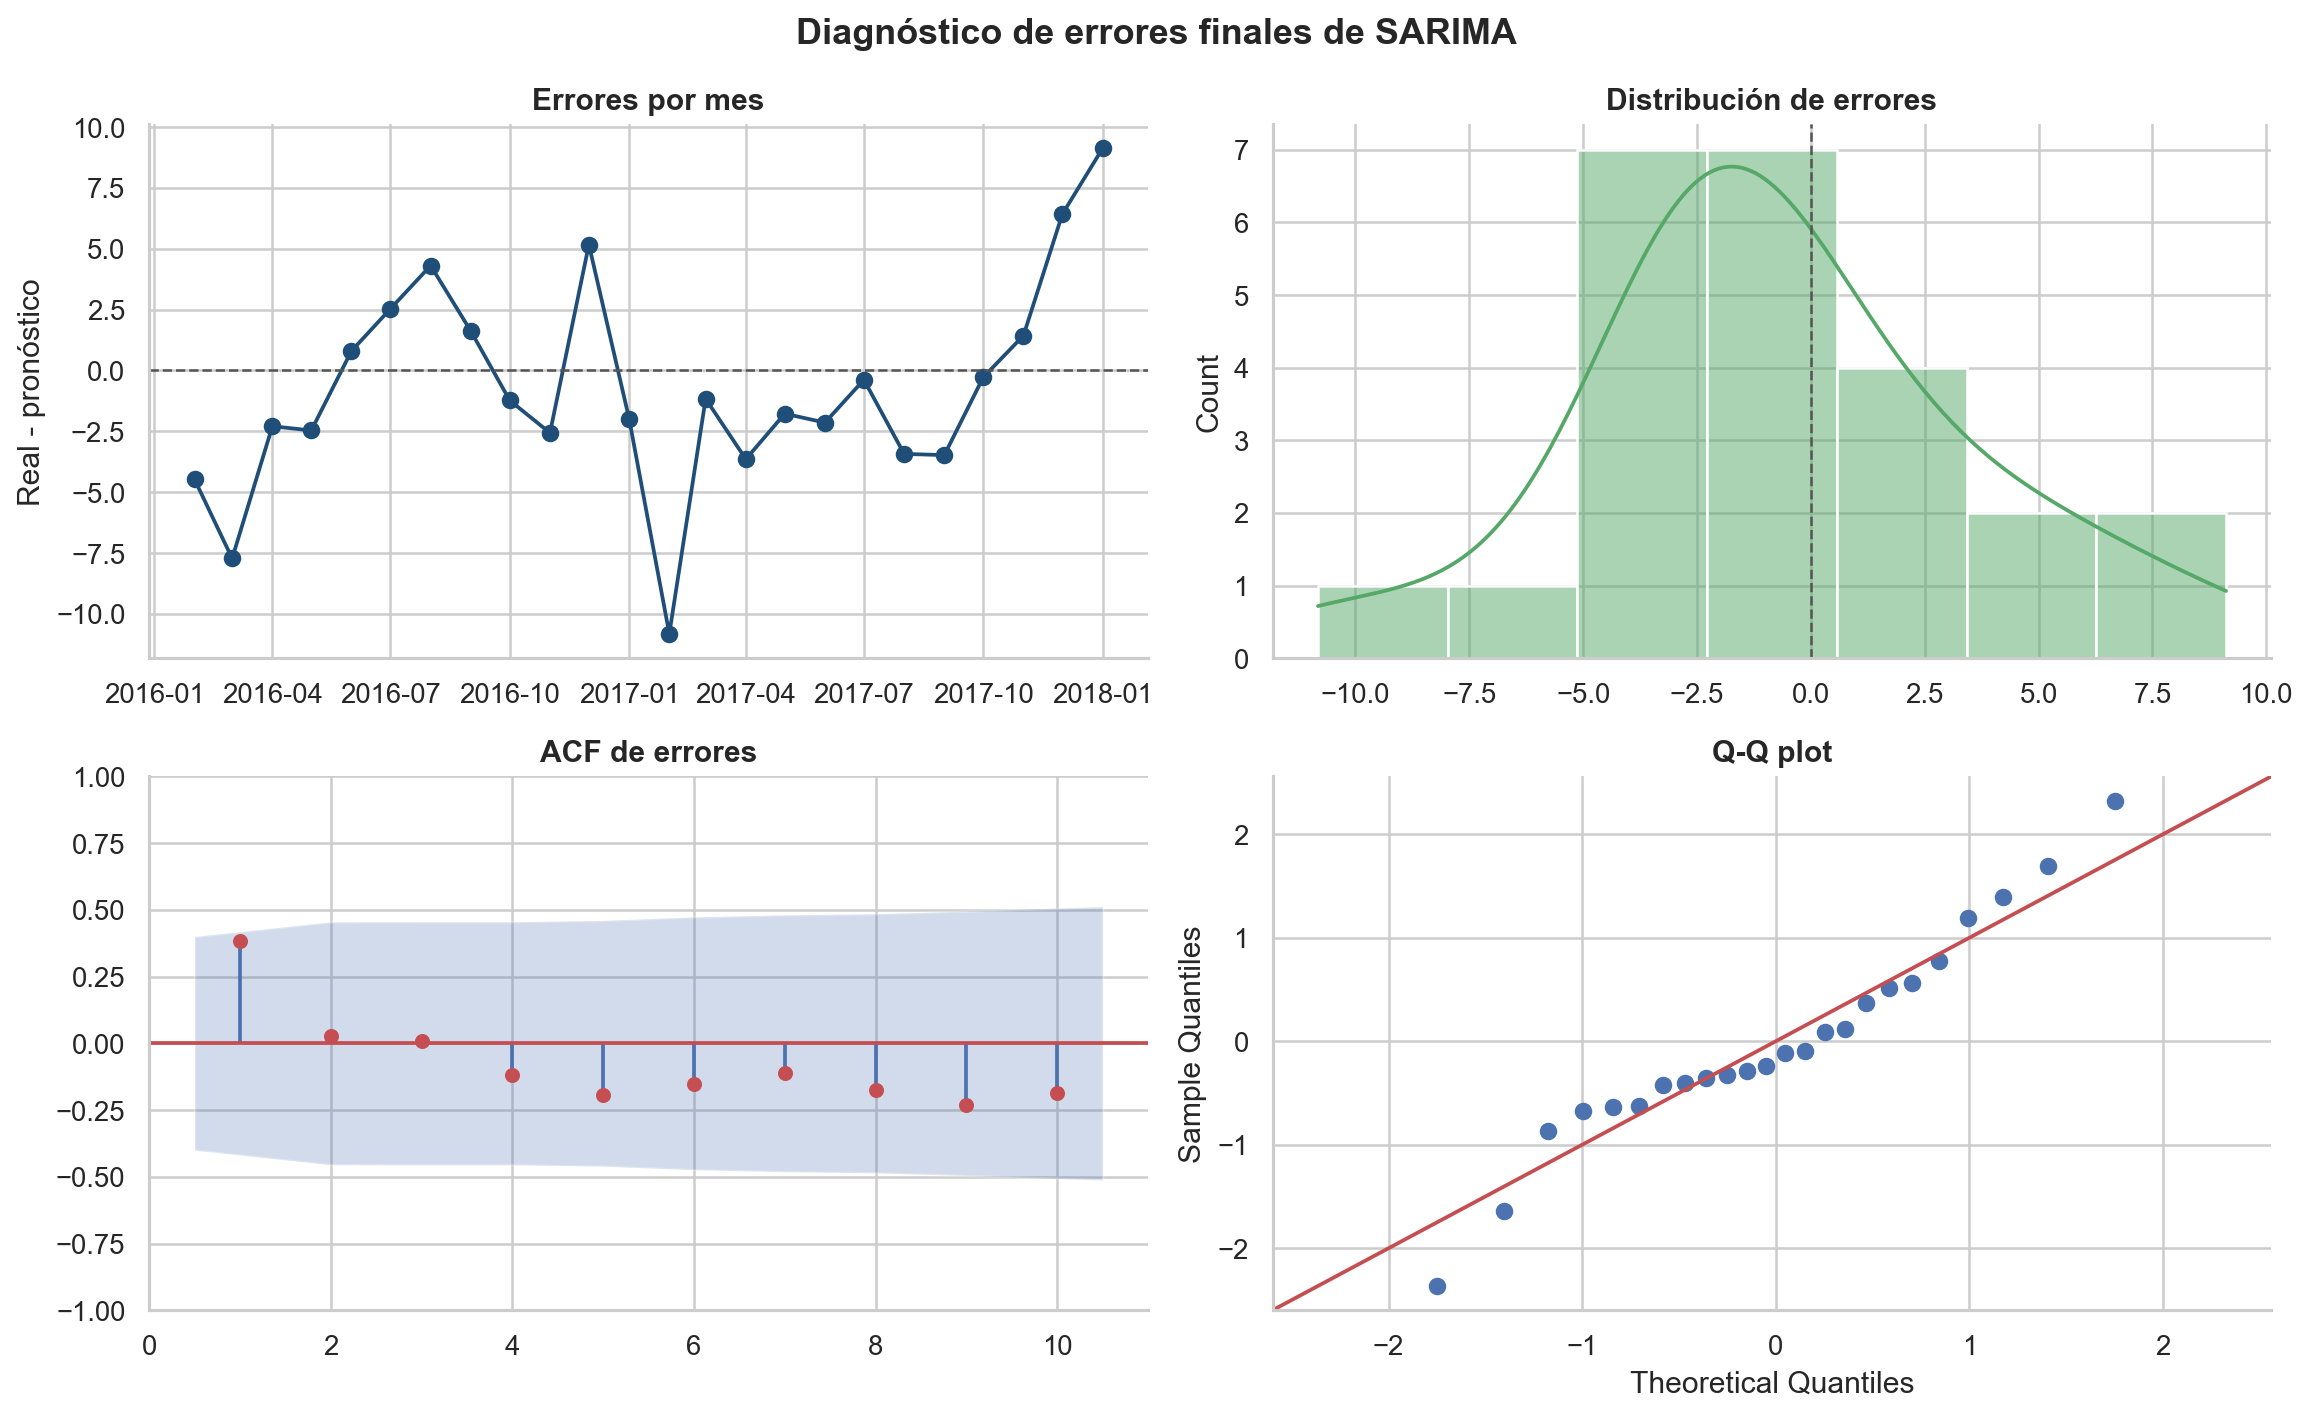
\includegraphics[width=\linewidth,height=0.66\paperheight,keepaspectratio]{15_sarima_errores_test.png}
    \column{0.27\textwidth}
      \begin{block}{Hallazgos}
        \begin{itemize}
          \item Error medio: \highlight{$-0,7713$}.
          \item Ljung--Box: $p=0,3696$ a 6 meses.
          \item Ljung--Box: $p=0,3818$ a 12 meses.
        \end{itemize}
      \end{block}
      \smallnote{No hay evidencia significativa de autocorrelación. Los desvíos de cola se interpretan con cautela: solo hay 24 errores.}
  \end{columns}
\end{frame}

% 10
\begin{frame}{Conclusiones}
  \begin{block}{Modelo recomendado}
    \centering
    \Large \highlight{$\mathrm{SARIMA}(2,0,2)(1,1,1)_{12}$}\par
    \normalsize Ajustado sobre $\log(y)$ · MAPE final: \textbf{3,3093\%}
  \end{block}

  \vspace{0.22cm}
  \begin{columns}[T,onlytextwidth]
    \column{0.31\textwidth}
      \textbf{Evidencia}
      \begin{itemize}
        \item Ganó en validation.
        \item Confirmó la ventaja en test.
        \item Superó claramente al baseline.
      \end{itemize}
    \column{0.31\textwidth}
      \textbf{Interpretación}
      \begin{itemize}
        \item La estacionalidad anual domina.
        \item SARIMA representa mejor esa estructura.
        \item XGBoost suaviza picos y valles.
      \end{itemize}
    \column{0.31\textwidth}
      \textbf{Límite}
      \begin{itemize}
        \item Horizonte final de 24 meses.
        \item Diagnóstico residual descriptivo.
        \item No se ajustó nada después de test.
      \end{itemize}
  \end{columns}

  \vfill
  \centering
  \color{Energy}\textbf{Una evaluación temporal justa sostuvo la misma conclusión en validation y test.}
\end{frame}

\end{document}
